\documentclass[12pt]{exam}
\usepackage{xkcdcolors}
\usepackage{tikz}
\usepackage[hidelinks]{hyperref}
\usepackage{wrapfig}
\usetikzlibrary {intersections,calc,through,angles,quotes}

\newsavebox{\mysolution}

\newenvironment{blanksolution}
  {%
    \begin{lrbox}{\mysolution}%
    \begin{minipage}{\linewidth}%
  }
  {%
    \end{minipage}%
    \end{lrbox}%
    \ifprintanswers
      \usebox{\mysolution}%
    \else
      \vspace{\dimexpr\ht\mysolution+\dp\mysolution\relax}%
    \fi
  }
\header{Geometric Constructions}{}{\today}
\firstpagefooter{}{}{\url{dishajk.github.io}}
\runningfooter{}{Page \thepage\ of \numpages}{}
\begin{document}
\section*{}
Reading suggestion: \emph{How to Solve it} by George P\'{o}lya
\section*{}
Recall Question 6 from the session on Sunday (20 Sep 2026), where you constructed a triangle given three of its measurements. We will use the following notation in all the exercises that follow.

\begin{figure}[h]
    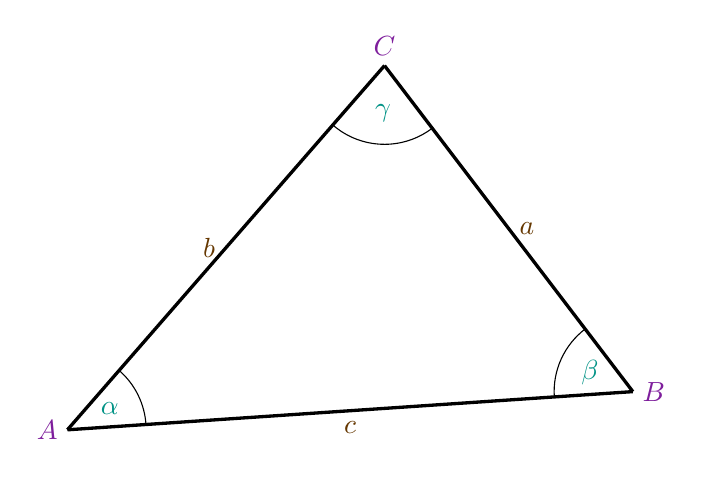
\begin{tikzpicture}
        \coordinate [label=left:\textcolor{xkcdPurple}{$A$}] (A) at ($ (0,0) + .5*(rand,rand) $);
        \coordinate [label=right:\textcolor{xkcdPurple}{$B$}] (B) at ($ (7.25,0.25) + .5*(rand,rand) $);
        \coordinate [label=90:\textcolor{xkcdPurple}{$C$}] (C) at ($ (3.5,5) + .5*(rand,rand) $);
        \draw[very thick,name path=c] (A) -- node[midway, below] {\textcolor{xkcdBrown}{$c$}} (B);
        \draw[very thick,name path=a] (B) -- node[midway, right] {\textcolor{xkcdBrown}{$a$}} (C);
        \draw[very thick,name path=b] (C) -- node[midway, left] {\textcolor{xkcdBrown}{$b$}} (A);

        \draw pic [draw, angle radius=1cm,"\textcolor{xkcdTeal}{$\alpha$}"] {angle = B--A--C};
        \draw pic [draw, angle radius=1cm,"\textcolor{xkcdTeal}{$\beta$}"] {angle = C--B--A};
        \draw pic [draw, angle radius=1cm,"\textcolor{xkcdTeal}{$\gamma$}"] {angle = A--C--B};
    \end{tikzpicture}
\end{figure}

The vertices of the triangle are \textcolor{xkcdPurple}{$A$}, \textcolor{xkcdPurple}{$B$}, and \textcolor{xkcdPurple}{$C$}. The sides opposite the vertices \textcolor{xkcdPurple}{$A$}, \textcolor{xkcdPurple}{$B$}, and \textcolor{xkcdPurple}{$C$} are denoted by \textcolor{xkcdBrown}{$a$}, \textcolor{xkcdBrown}{$b$}, and \textcolor{xkcdBrown}{$c$}, respectively. The angles at \textcolor{xkcdPurple}{$A$}, \textcolor{xkcdPurple}{$B$}, and \textcolor{xkcdPurple}{$C$} are denoted by \textcolor{xkcdTeal}{$\alpha$}, \textcolor{xkcdTeal}{$\beta$}, and \textcolor{xkcdTeal}{$\gamma$}, respectively.

\begin{figure}[h]
    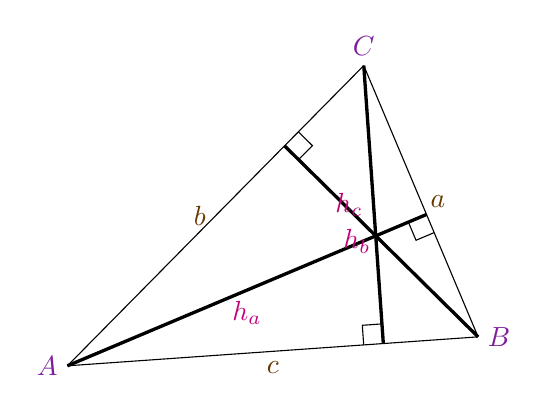
\begin{tikzpicture}
        \coordinate [label=left:\textcolor{xkcdPurple}{$A$}] (A) at ($ (0,0) + .25*(rand,rand) $);
        \coordinate [label=right:\textcolor{xkcdPurple}{$B$}] (B) at ($ (5.25,0.25) + .25*(rand,rand) $);
        \coordinate [label=90:\textcolor{xkcdPurple}{$C$}] (C) at ($ (3.5,4) + .25*(rand,rand) $);
        \draw[name path=c] (A) -- node[midway, below] {\textcolor{xkcdBrown}{$c$}} (B);
        \draw[name path=a] (B) -- node[midway, right] {\textcolor{xkcdBrown}{$a$}} (C);
        \draw[name path=b] (C) -- node[midway, left] {\textcolor{xkcdBrown}{$b$}} (A);

        \coordinate (Ha) at ($(B)!(A)!(C)$);
        \coordinate (Hb) at ($(C)!(B)!(A)$);
        \coordinate (Hc) at ($(A)!(C)!(B)$);
        \draw[very thick] (A) -- (Ha) node[midway,below] {\textcolor{xkcdMagenta}{$h_a$}}; 
        \draw pic [draw, angle radius=0.25cm] {right angle = A--Ha--B}; 
        \draw[very thick] (B) -- (Hb) node[midway,left] {\textcolor{xkcdMagenta}{$h_b$}};  
        \draw pic [draw, angle radius=0.25cm] {right angle = B--Hb--C}; 
        \draw[very thick] (C) -- (Hc) node[midway,left] {\textcolor{xkcdMagenta}{$h_c$}};  
        \draw pic [draw, angle radius=0.25cm] {right angle = C--Hc--A}; 
    \end{tikzpicture}
\end{figure}

The altitude (or height measured from) from \textcolor{xkcdPurple}{$A$} to the side \textcolor{xkcdBrown}{$a$} (line segment $BC$) is denoted by \textcolor{xkcdMagenta}{$h_a$}, and so on.

\begin{figure}[h]
    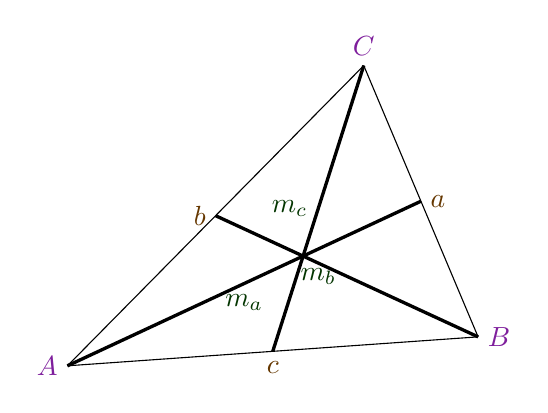
\begin{tikzpicture}
        \coordinate [label=left:\textcolor{xkcdPurple}{$A$}] (A) at ($ (0,0) + .25*(rand,rand) $);
        \coordinate [label=right:\textcolor{xkcdPurple}{$B$}] (B) at ($ (5.25,0.25) + .25*(rand,rand) $);
        \coordinate [label=90:\textcolor{xkcdPurple}{$C$}] (C) at ($ (3.5,4) + .25*(rand,rand) $);
        \draw[name path=c] (A) -- node[midway, below] {\textcolor{xkcdBrown}{$c$}} (B);
        \draw[name path=a] (B) -- node[midway, right] {\textcolor{xkcdBrown}{$a$}} (C);
        \draw[name path=b] (C) -- node[midway, left] {\textcolor{xkcdBrown}{$b$}} (A);

        \coordinate (Ma) at ($(B)!0.5!(C)$);
        \coordinate (Mb) at ($(C)!0.5!(A)$);
        \coordinate (Mc) at ($(A)!0.5!(B)$);
        \draw[very thick] (A) -- (Ma) node[midway,below] {\textcolor{xkcdDarkGreen}{$m_a$}}; 
        \draw[very thick] (B) -- (Mb) node[midway,left] {\textcolor{xkcdDarkGreen}{$m_b$}};  
        \draw[very thick] (C) -- (Mc) node[midway,left] {\textcolor{xkcdDarkGreen}{$m_c$}};
    \end{tikzpicture}
\end{figure}

The median from \textcolor{xkcdPurple}{$A$} to the side \textcolor{xkcdBrown}{$a$} is \textcolor{xkcdDarkGreen}{$m_a$}, and so on.

The angle bisector of \textcolor{xkcdTeal}{$\alpha$} to the side \textcolor{xkcdBrown}{$a$} is \textcolor{xkcdDarkBlue}{$d_{\alpha}$}, and so on. 

The radius of the circumscribed circle is $R$, and the radius of the inscribed circle is $r$.

In the following exercises, it may not always be possible to construct a triangle satisfying the given conditions. For example, try to construct a triangle with $a=4$, $b=5$, and $c=10$. If you are unable to construct it, explain why the triangle is not possible.

Remember to break each problem down into smaller problems, as we did during the session. It may be helpful to write down your construction steps as you work.

Have fun constructing!


\begin{questions}
    \question Construct a triangle given $a$, $m_a$, and $b$
    \question Construct a triangle given $a$, $m_a$, and $h_a$
    \question Construct a triangle given $a$, $\alpha$, and $h_a$
    \question Construct a triangle given $a$, $\alpha$, and $m_a$
    \question Construct a triangle given $a$, $\alpha$, and $r$
    \question Construct a triangle given $a$, $c$, and $h_b$
    \question Construct a triangle given $a$, $d_{\gamma}$, and $h_b$
    \question Construct a triangle given $h_a$, $\beta$, and $h_b$
    \question Construct a triangle given $\alpha$, $\beta$, and $d_{\gamma}$
    \question Construct a triangle given $h_a$, $h_b$, and $h_c$
    \question Construct a triangle given $a$, $\alpha$, and $R$
\end{questions}

\end{document}
\question Construct the perpendicular bisector of the line given below

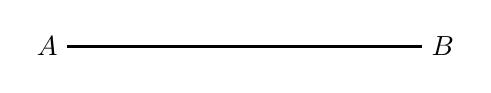
\begin{tikzpicture}
        \coordinate [label=left:$A$] (A) at (0,0);
        \coordinate [label=right:$B$] (B) at (4.5,0);
        \draw[very thick] (A) -- (B);
\end{tikzpicture}
\begin{parts}
        \part unknown:
        \begin{blanksolution}
           $CE$, the perpendicular bisector of $AB$
        \end{blanksolution}
        \part data:
          \begin{blanksolution}
            points $A$ and $B$
        \end{blanksolution}
        \part condition:
        \begin{blanksolution}
            $AD = DB$ and $CE \perp AB$ 
        \end{blanksolution}
    \end{parts}
    \begin{solution}
        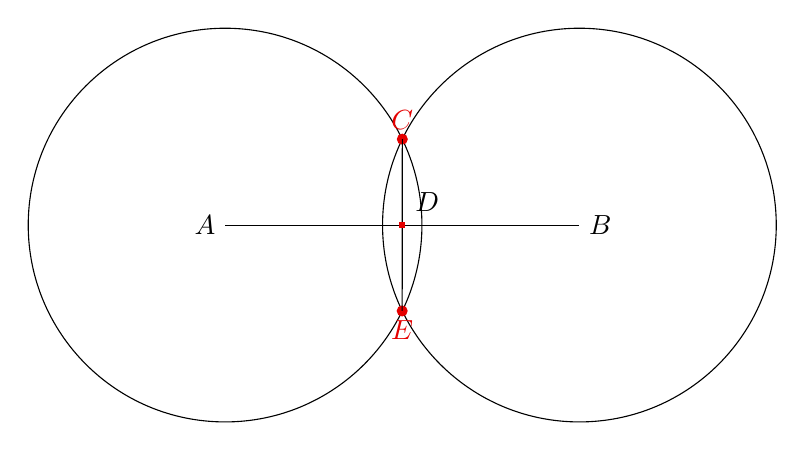
\begin{tikzpicture}
        \coordinate [label=left:$A$] (A) at (0,0);
        \coordinate [label=right:$B$] (B) at (4.5,0);
        \draw[name path=A--B] (A) -- (B);

        \draw[name path=r] (B) circle [radius=2.5];
        \draw[name path=l] (A) circle [radius=2.5];

        \fill [xkcdRed,name intersections={of=r and l, by = {[label=90:$C$]C,[label=-90:$E$]E}}] 
        (C) circle (2pt)
        (E) circle (2pt);

        \draw [name path=C--E] (C) -- (E);
        \path [name intersections={of=A--B and C--E,by=D}];
        \node [fill=xkcdRed,inner sep=1pt,label=45:$D$] at (D) {};
\end{tikzpicture}
    \end{solution}

\question Circumscribe a circle about the triangle given below

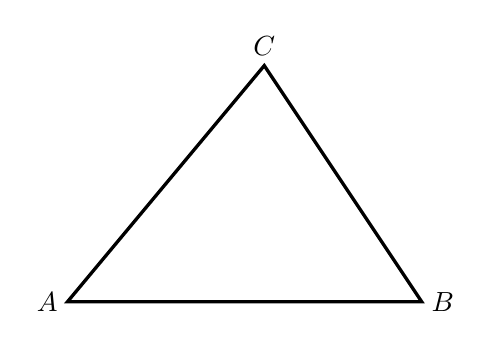
\begin{tikzpicture}
        \coordinate [label=left:$A$] (A) at (0,0);
        \coordinate [label=right:$B$] (B) at (4.5,0);
        \coordinate [label=above:$C$] (C) at (2.5,3);
        \draw[very thick] (A) -- (B) -- (C) -- cycle;
    \end{tikzpicture}
    \begin{parts}
        \part unknown:
        \begin{blanksolution}
            $X$ the centre of the Circle
        \end{blanksolution}
        \part data:
          \begin{blanksolution}
            points $A$, $B$, and $C$
        \end{blanksolution}
        \part condition:
        \begin{blanksolution}
            $XA=XB=XC$
        \end{blanksolution}
    \end{parts}

    \begin{blanksolution}
        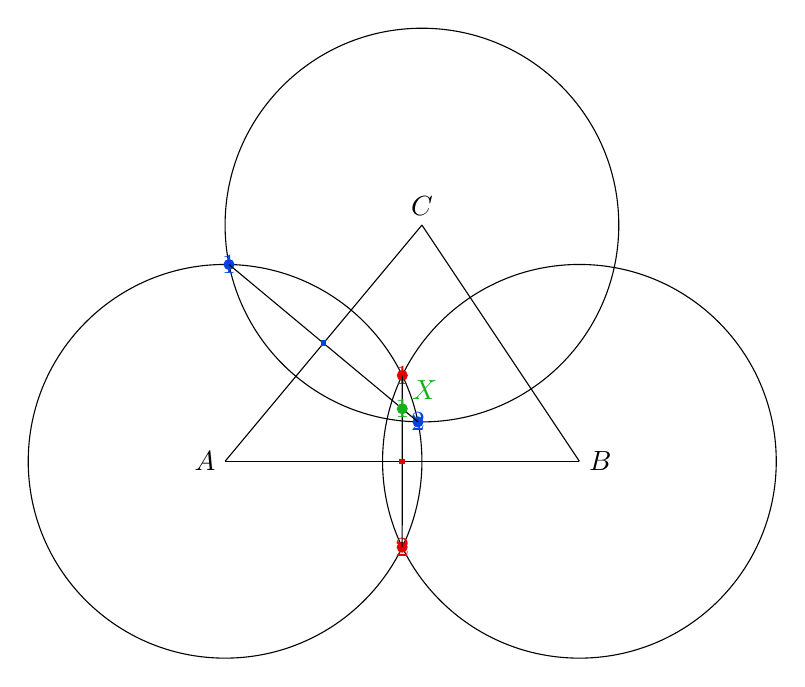
\begin{tikzpicture}
        \coordinate [label=left:$A$] (A) at (0,0);
        \coordinate [label=right:$B$] (B) at (4.5,0);
        \coordinate [label=above:$C$] (C) at (2.5,3);
        \draw[name path=A--B] (A) -- (B);
        \draw (B) -- (C);
        \draw[name path=A--C] (A) -- (C);

        \draw[name path=r] (B) circle [radius=2.5];
        \draw[name path=l] (A) circle [radius=2.5];
        \fill [xkcdRed,name intersections={of=r and l, by = {C1,C2}}] 
        (C1) circle (2pt) node {1}
        (C2) circle (2pt) node {2};

        \draw [name path=C1--C2] (C1) -- (C2);
        \path [name intersections={of=A--B and C1--C2,by=D}];
        \node [fill=xkcdRed,inner sep=1pt] at (D) {};

        \draw[name path=t] (C) circle [radius=2.5];
        \fill [xkcdBlue,name intersections={of=l and t, by = {B1,B2}}] 
        (B1) circle (2pt) node {1}
        (B2) circle (2pt) node {2};

        \draw [name path=B1--B2] (B1) -- (B2);
        \path [name intersections={of=A--C and B1--B2,by=E}];
        \node [fill=xkcdBlue,inner sep=1pt] at (E) {};

        \fill [xkcdGreen,name intersections={of=B1--B2 and C1--C2, by = {[label=45:$X$]X}}] 
        (X) circle (2pt) node {1};
    \end{tikzpicture}

    \end{blanksolution}
    \question Find the locus of points that are equidistant from two given lines.

    \question Inscribe a circle in the triangle given below

    \begin{tikzpicture}
        \coordinate [label=left:$A$] (A) at (0,0);
        \coordinate [label=right:$B$] (B) at (8.5,0);
        \coordinate [label=above:$C$] (C) at (4,5);
        \draw[very thick] (A) -- node[midway, below] {$c$} (B) -- node[midway, right] {$a$} (C) -- node[midway, left] {$b$} cycle;
    \end{tikzpicture}

    \begin{parts}
        \part unknown:
        \begin{blanksolution}
            $X$ the centre of the Circle
        \end{blanksolution}
        \part data:
          \begin{blanksolution}
            lines $a$, $b$, and $c$
        \end{blanksolution}
        \part condition:
        \begin{blanksolution}
            $X$ is at the same distance from lines $a$, $b$, and $c$
        \end{blanksolution}
    \end{parts}

So this exercise is mainly going to be to help you understand problem solving

Problem describe, or let's construct a triangle being given its three sides

So what I want you to do first is list all the given as in what is noon. Okay as in like if there is no known if there is no unknown, then we don't have to like there is no problem to solve right so in this problem, the unknown is the geometry figure, which is the right triangle so we are going to call the given as the data and what's the data we have for the first question, I'm going to give you all the three sides, the value of all the three sides, so the sheet you have three lines